\section{Implementation}

This chapter describes how the system specified in the Approach chapter (\S4) is built: the codebase layout, the data-engineering pipeline, the front-end visualisation components, the linked-view brushing implementation, and any design-decision deviations encountered during construction.

\subsection{System Architecture and Codebase Layout}

The repository is laid out around an artefact-first workflow: each named directory holds one class of project artefact --- raw and processed data with tracked dictionary/provenance/data-quality sidecars, the executed exploratory notebooks behind the \S1.1 statistics, the production \path{src/} package split into data pipelines, Flask API, and D3 dashboard, the pytest harness, the LaTeX report, the literature base, and the evaluation records --- and every prose claim in this report is traceable to a file in one of these locations. Appendix~A indexes the individual entry points, so the body of this chapter concentrates on design decisions and their verification rather than on file-by-file description.

The implemented artefact includes the backend (\S5.3), the D3 front-end (\S5.4), the assignment-footprint data layer and API (\S5.5), the mobilisation join, dashboard screenshot captures, and the published station-address proximity recovery (\S5.6 D1). The front-end UI toggle for the footprint scenario is planned as future work.

\begin{figure}[h]
\centering
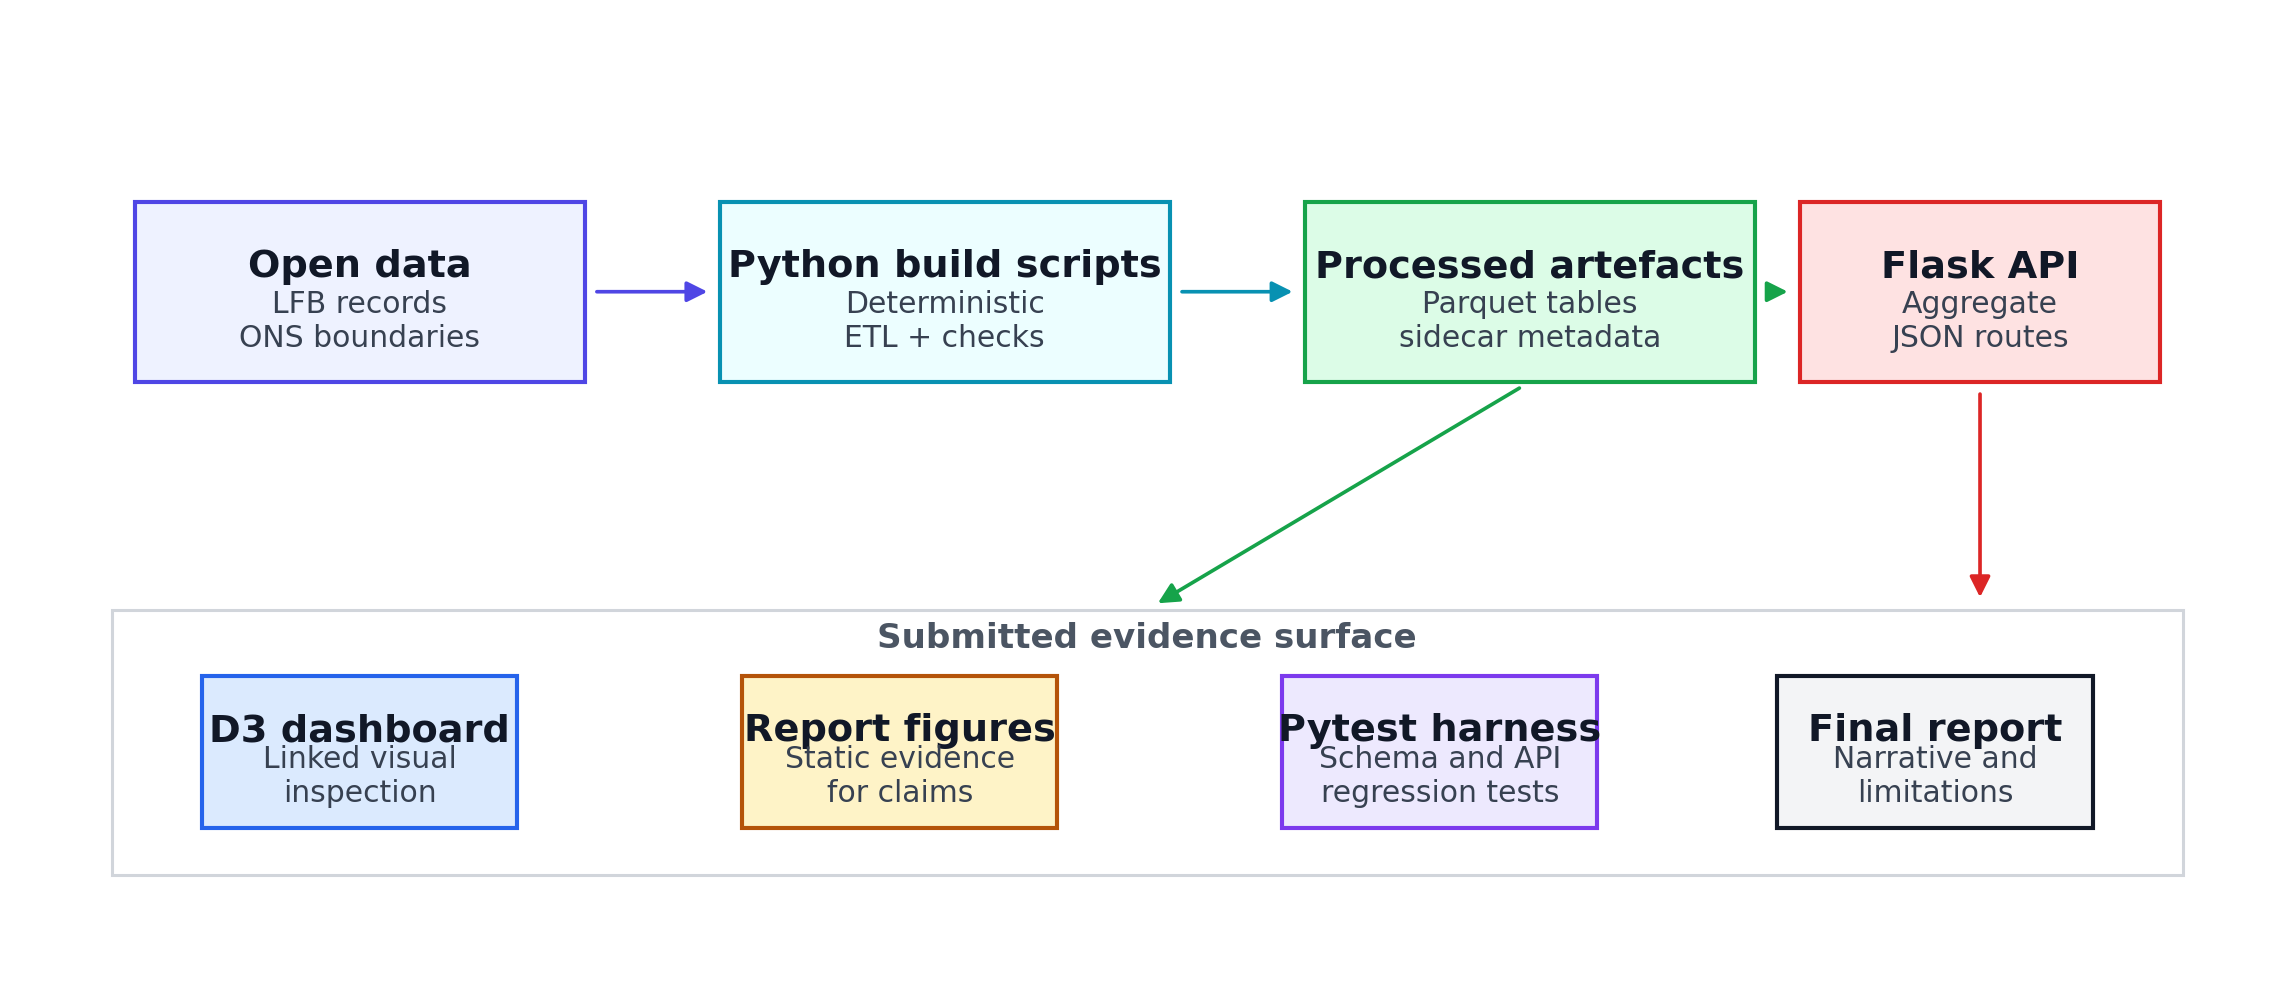
\includegraphics[width=\textwidth]{figures/architecture/fig_system_architecture_overview.png}
\caption{System architecture overview. The figure summarises the concrete implementation path from open LFB/ONS data through Python build scripts and auditable artefacts to the Flask API, D3 dashboard, and report evidence; it is a system schematic, not a data result.}
\label{fig:implementation-pipeline}
\end{figure}

\begin{figure}[h]
\centering
\small
\resizebox{\textwidth}{!}{%
\begin{tikzpicture}[
    node distance=7mm and 9mm,
    box/.style={draw, rounded corners=1.5pt, align=center, text width=3.0cm, minimum height=0.9cm, fill=gray!8},
    server/.style={box, fill=blue!8, draw=blue!55!black},
    client/.style={box, fill=green!8, draw=green!50!black},
    contract/.style={box, fill=orange!9, draw=orange!65!black},
    arr/.style={-{Stealth[length=2.0mm]}, line width=0.45pt}
]
\node[server] (factory) {Flask\\\texttt{create\_app}};
\node[server, right=of factory] (frame) {in-memory\\summary frames};
\node[contract, right=of frame] (api) {JSON routes\\filters + caveats};
\node[client, right=of api] (state) {\texttt{dashboard.js}\\shared state};
\node[client, below=of state] (views) {D3 renderers\\map / trend / table};
\node[contract, below=of api] (assets) {same-origin\\static assets};
\draw[arr] (factory) -- (frame);
\draw[arr] (frame) -- (api);
\draw[arr] (api) -- (state);
\draw[arr] (state) -- (views);
\draw[arr] (factory) |- (assets);
\draw[arr] (assets) -- (views);
\draw[arr] (views.east) -- ++(0.45,0) |- (state.east);
\end{tikzpicture}}
\caption{Runtime component boundary for the Flask/D3 implementation, showing the server-side data contract, client-side shared state, and linked D3 renderers.}
\label{fig:runtime-component-boundary}
\end{figure}

\subsection{Data Pipeline}

\begin{figure}[H]
\centering
\small
\resizebox{\textwidth}{!}{%
\begin{tikzpicture}[
    node distance=6mm and 7mm,
    box/.style={draw, rounded corners=1.5pt, align=center, text width=3.0cm, minimum height=0.86cm, fill=gray!8},
    raw/.style={box, fill=blue!8, draw=blue!55!black},
    artefact/.style={box, fill=green!8, draw=green!50!black},
    output/.style={box, fill=orange!9, draw=orange!65!black},
    arr/.style={-{Stealth[length=2.0mm]}, line width=0.45pt}
]
\node[raw] (incidents) {LFB Incident\\Records};
\node[raw, below=of incidents] (mobilisations) {LFB Mobilisation\\Records};
\node[raw, below=of mobilisations] (boundaries) {ONS borough\\boundaries};
\node[raw, below=of boundaries] (stations) {Public station-address\\postcode table};

\node[artefact, right=1.2cm of incidents] (canonical) {Canonical incident\\artefact\\dictionary / provenance / DQ memo};
\node[artefact, right=1.2cm of canonical] (summary) {Borough-month-\\incident-group\\summary};
\node[artefact, below=of summary] (matched) {Matched mobilisation\\artefact};
\node[artefact, below=of matched] (footprints) {Assignment-footprint\\centroids};
\node[artefact, below=of footprints] (d1) {Public station-address\\recovery / D1\\comparison};

\node[output, right=1.2cm of summary] (api) {Flask API};
\node[output, below=of api] (dashboard) {D3 dashboard};
\node[output, below=of dashboard] (figures) {Report figures};
\node[output, below=of figures] (eval) {Evaluation\\artefacts};

\draw[arr] (incidents.east) -- (canonical.west);
\draw[arr] (boundaries.east) -- ++(0.25,0) |- ([yshift=9mm]api.north) -- (api.north);
\draw[arr] (canonical.east) -- (summary.west);
\draw[arr] (canonical.east) -- ++(0.35,0) |- (matched.west);
\draw[arr] (mobilisations.east) -- ++(0.45,0) |- (matched.west);
\draw[arr] (canonical.east) -- ++(0.35,0) |- (footprints.west);
\draw[arr] (stations.east) -- ++(0.45,0) |- (d1.west);
\draw[arr] (footprints.south) -- (d1.north);
\draw[arr] (summary.east) -- (api.west);
\draw[arr] (matched.east) -- ++(0.45,0) |- (figures.west);
\draw[arr] (d1.east) -- ++(0.45,0) |- (figures.west);
\draw[arr] (api.south) -- (dashboard.north);
\draw[arr] (dashboard.south) -- (figures.north);
\draw[arr] (figures.south) -- (eval.north);
\end{tikzpicture}}
\caption{Deterministic data artefact dependency graph. The figure shows the implemented pipeline dependencies from raw open-data inputs to submitted dashboard/report artefacts; it is a pipeline schematic, not a data result.}
\label{fig:data-artefact-dependency-graph}
\end{figure}

\subsubsection{Goal and Acceptance Criteria}
The data pipeline produces a single canonical analytic artefact, \path{data/processed/lfb_canonical_2024_2026.parquet}, that all downstream notebooks, the dashboard backend (\S5.3), and the prose statistics in \S1.1 read from. The build contract is deliberately auditable: the script is rerunnable on the same input, emits the parquet, dictionary, provenance JSON and data-quality memo, and fails on automated validation checks when published-statistic invariants drift.

\subsubsection{Ingestion and Transformations}
The single entry point \path{src/data/build_canonical.py} reads the 66\,MB source workbook (293{,}646 rows $\times$ 39 columns) and applies the explicit cleaning decisions in Table~\ref{tab:canonical-cleaning}. The process does not impute unavailable values or discard records: the canonical output retains 293{,}646 rows and carries missingness and validity as auditable fields.

\begin{table}[H]
\centering
\footnotesize
\begin{tabularx}{\textwidth}{>{\raggedright\arraybackslash}p{2.6cm}>{\raggedright\arraybackslash}X>{\raggedright\arraybackslash}X}
\toprule
Raw-data issue & Cleaning decision & Retained audit signal \\
\midrule
Mixed date/time types & Parse with coercion; derive month, weekday, weekend, and hour partitions & Invalid values remain null in typed columns \\
Ambiguous response-time unit and missing values & Coerce to numeric seconds, derive minutes, and use a nullable six-minute flag & Missing times are excluded from the recorded-time denominator, never coded as non-exceedances \\
Precise and rounded coordinates coexist & Coerce for Greater-London bounding-box checks; do not impute precise points & Separate \path{coord_precise_valid} and \path{coord_rounded_valid} flags \\
Inconsistent borough capitalisation & Trim and title-case into \path{borough_canonical} & Original name and canonical name are both retained \\
Potential silent row loss & Preserve every source row and assert input/output counts & 293{,}646-row invariant plus data-quality memo \\
\bottomrule
\end{tabularx}
\caption{Canonical incident-data cleaning decisions implemented in \texttt{build\_canonical.py}.}
\label{tab:canonical-cleaning}
\end{table}

\subsubsection{Provenance, Dictionary, and DQ Memo}
Three sidecar files are emitted next to the parquet. The provenance JSON records source filename, SHA-256 hash, UTC extraction timestamp, transformations, constants, and output columns. The dictionary records dtype, non-null count, source, and notes for each column. The DQ memo restates the headline numbers cited in \S1.1 and lists four limitations the dashboard must surface rather than hide. Together, the canonical parquet and sidecars let a reviewer audit the 50-column schema, headline statistics, and transformation record without the 66\,MB input file present locally.

\subsubsection{Automated Validation Checks and Reproducibility Guard-Rail}
The build emits a non-zero exit when schema, unit, coordinate-coverage, exceedance-share, or incident-group sanity bands fail. These checks include a response-time unit band, precise/rounded coordinate coverage bands, the recorded-time exceedance denominator, and the False Alarm share. Should the LFB schema change in a future release, the build will force a code-level reconciliation before downstream work proceeds rather than allowing silent drift. The detailed invariant matrix is consolidated in Appendix~A.

\subsubsection{Second-Stage Aggregation: Borough Monthly Summary}
A second pipeline script, \path{src/data/build_borough_summary.py}, pre-aggregates 2{,}574 borough--month--incident-group cells. Its 20 columns include exact recorded/exceedance counts, the author-derived share above 360 seconds, a two-sided 95\% Wilson interval, a recorded-$n<30$ display flag, and a partial-month flag, alongside response percentiles and audit fields. The final-month flag is derived from the source maximum date (27 February 2026), not entered in the front end. Pre-aggregation reduces each dashboard request from a 293{,}646-row \path{groupby} to a 2{,}574-row lookup.

\subsubsection{External Verification Harness}
The build-time validation checks are the \emph{author's} guard against pipeline regressions; the \path{tests/} directory adds an \emph{external} pytest harness, one module per artefact, that any reviewer can run with \texttt{python -m pytest tests/}. The suite verifies schema contracts, published-baseline bands, cross-artefact consistency, API behaviour, footprint negative paths, and station-location invariants, including a dedicated regression test for the \path{exceeds_six_min_share} denominator. Appendix~A gives the consolidated test matrix so the implementation chapter need not enumerate every assertion.

\subsubsection{Published Station-Address Proximity Recovery}
The D1 recovery script reads the June 2017 low-carbon-generator file from London Datastore; the source page describes its LFEPA entries as correct to June 2016~\cite{lfb_stations}. It geocodes the 104 historical address rows to postcode centroids through postcodes.io~\cite{postcodesio}. Of these rows, 102 names match the distinct assignment-footprint labels in the 2024--2026 incident slice; two do not. These counts describe different artefacts and neither is presented as a current operating-station total. The matched comparison has a median address-to-footprint shift of 0.43\,km and p90 of 0.99\,km, confirming that a footprint centroid is not a building location.

\subsection{Backend API}

\subsubsection{Scope and Design Boundary}
The backend exposes a JSON HTTP API to the D3 front end (\S5.4) over the borough-summary parquet of \S5.2. The first-release scope is deliberately narrow: a single resource endpoint, \texttt{GET} \path{/api/borough_summary}, a \texttt{GET} \path{/api/borough_boundaries} boundary layer for the choropleth, plus a \texttt{GET} \path{/health} liveness check. The dashboard's borough drill-down view requires no per-incident detail, so the backend never exposes the 293{,}646-row canonical incident table through any route; restricting the public surface to aggregations of \S5.2 keeps the unfiltered summary payload to about 1.0\,MiB (and typical selected-borough payloads to about 31\,KiB) while preserving a defensible privacy posture because no precise per-incident coordinates leave the backend through this interface.

\subsubsection{Endpoint Contract}
\texttt{GET} \path{/api/borough_summary} accepts the three group-key filters \path{borough_canonical}, \path{year_month}, and \path{IncidentGroup}. Repeated values are treated as within-column unions and combinations across parameters are intersected. The response contains \path{rows}, \path{row_count}, and \path{filters_applied}; row keys mirror the borough-summary parquet schema documented in \path{docs/API_CONTRACT.md}. Unknown filter keys are rejected with HTTP 400 and an enumerated allow-list of valid keys; unknown filter \emph{values} return HTTP 200 with an empty \path{rows} array because an empty selection is a legitimate analytical state.

\subsubsection{Implementation Details}
The Flask application is constructed through the \path{create_app(parquet_path=None)} factory, which loads the borough-summary parquet once at app-creation time and binds the resulting pandas \path{DataFrame} into the route handlers via closure; subsequent requests filter the in-memory frame and serialise the matched rows. Measured on the 2{,}574-row borough summary on a single 16\,GB MacBook (no caching layer, no concurrent load), the response time averages 1.1\,ms for a single-borough filtered request and 17.7\,ms for the worst-case unfiltered full-dataset response over 100 sequential requests; this comfortably meets the linked-view brushing budget of \S5.4 and removes the need for an external store at this stage. Two pandas-to-JSON conversion issues are handled centrally in \path{_row_to_jsonable}: pandas float \path{NaN} is not JSON-serialisable per RFC 8259 and is converted to JSON \path{null}, and the nullable-boolean \path{exceeds_six_min_target} sentinel \path{pd.NA} is similarly converted, so the front end can rely on JSON \path{null} as the single missing-value token.

\subsubsection{API Verification Harness}
\path{tests/test_api.py} adds fourteen endpoint-level tests on top of the data-pipeline tests of \S5.2, covering the liveness route, the unfiltered and filtered summary contracts, exact response-schema matching against the parquet column set, filter round-trips, intersections, and repeated-key unions, the deliberate empty-result-versus-HTTP-400 distinction, JSON \path{NaN} safety, and the reachability of the dashboard assets and boundary route. All fourteen pass under the validation command \texttt{python -m pytest tests/ -q}.

\subsection{Front-End: Linked Views and Uncertainty-Aware Encodings}

The first front-end slice is a static D3 module \cite{bostock2011} served by the same Flask app, rather than a separate React/Vite build. This is a deliberate maintenance choice for the thesis artefact: the interface has one primary dashboard screen, the data are already pre-aggregated, and same-origin serving avoids cross-origin configuration while keeping the project faithful to the planned Flask + D3.js stack of \S4.3. The front-end files live under \path{src/dashboard/}: \path{index.html} defines the dashboard shell and native controls; \path{styles.css} defines the compact operational visual language (white surfaces, charcoal text, teal response-performance encoding, amber target-threshold cueing); and \path{dashboard.js} owns data loading, state, D3 rendering via the declarative \texttt{enter/update/exit} pattern \cite{bostock2011, heer2010}, and linked interactions.

At load time the browser fetches two same-origin resources: \path{/api/borough_summary} for the 2{,}574 aggregate rows and \path{/api/borough_boundaries} for the 33-feature GLA London Borough GeoJSON layer. The boundary file is tracked as \path{data/processed/london_borough_boundaries.geojson} with a provenance sidecar recording the GLA ArcGIS service URL and download method; joining is performed case-insensitively because the canonical LFB pipeline title-cases particles such as ``and''/``of'' while the GLA boundary names do not. The dashboard state is the triple \emph{borough, month, incident group}. Changing any select control, clicking a borough on the map, or clicking a row in the ranking table updates that shared state and re-renders all linked panels --- the \emph{Connect} interaction category of \cite{yi2007} operationalising the \emph{relate} task of Shneiderman's mantra \cite{shneiderman1996}.

The current screen contains four linked views. The borough map and ranking table encode the author-derived share above 360 seconds; hover and table rows show the recorded denominator and 95\% Wilson interval, with a warning below 30 recorded times. The trend marks February 2026 as partial, while the distribution panel shows median-to-p95 variability and a six-minute reference line. Precise-coordinate availability was removed from the borough ranking because the aggregate uses the published borough field; coordinate coverage remains report-side evidence for point-level maps.

\subsection{Assignment-Footprint Proxy}

\subsubsection{Scope and Naming}
The station-context design of \S4.5 requires the implementation to keep two things separate: station-related evidence that can be supported from open data, and routing-grade coverage evidence that cannot. The first-iteration artefact described below implements the supported half as an \emph{assignment-footprint proxy}, derived entirely from the canonical incident table with no external station-locations dataset. The wording change is load-bearing: a coverage proxy in the OR sense (\S\ref{sec:lit-optimisation}) compares geographic regions against fixed station building locations and dispatch travel times; what this artefact compares is the centroid of where each station's incidents historically happened against the centroid of where each borough's incidents historically happened. \S5.6 records the narrower implementation choice as an explicit deviation against N1 and names the public-address recovery path.

\subsubsection{Data Layer}
Two scripts derive assignment-footprint and borough-demand anchors from rounded incident coordinates. \path{src/data/build_station_locations.py} groups by \path{IncidentStationGround}; its 102 rows are distinct source labels, not verified buildings. \path{src/data/build_borough_centroids.py} groups by \path{borough_canonical}. Their medians are transparent spatial proxies, but rounded-coordinate displacement and the common incident source prevent routing, coverage, or current-estate claims.

\subsubsection{Footprint-Scenario API}
Two Flask endpoints expose the artefact. \texttt{GET} \path{/api/station_footprints} returns the 102 assignment-footprint labels; \texttt{GET} \path{/api/footprint_scenario?remove=...} removes named footprint labels and recomputes the nearest remaining footprint. Formally, writing $S$ for the retained label set with footprint centroids $f_s$ and $c_b$ for the demand centroid of borough $b$,
\begin{equation}
d_b(S) \;=\; \min_{s \in S} \bigl\| c_b - f_s \bigr\|_2,
\qquad
d_b(S \setminus X) \;\ge\; d_b(S) \quad \forall\, X \subset S,
\label{eq:footprint-monotonicity}
\end{equation}
so a removal can only delete minimisation candidates, and the nearest-footprint distance is non-decreasing under any scenario. The endpoint name uses ``footprint'' rather than ``coverage'' because the underlying anchors are footprint centroids, not station building locations; the same name change is applied throughout the prose to signal that the result is an assignment shift, not a coverage decrement. Three negative paths fail with HTTP 400 rather than silently returning a misleading result: an unknown query key, a \path{remove} value that names a station not in the dataset, and a removal list that empties the entire station set. The disclaimer of \S4.5, expanded to spell out the footprint-not-coverage framing and to point at the \S5.6 deviation, is attached verbatim to every response payload so that any downstream consumer (dashboard, screenshot, copied JSON) carries the framing.

\subsubsection{Verification of the Footprint-Scenario API}
Six endpoint tests in \path{tests/test_api.py} carry the contract into the test suite: the footprint table and baseline scenario return their required schemas with the disclaimer attached; removing any real station never decreases any borough's nearest-footprint distance (the monotonicity invariant of Eq.~\ref{eq:footprint-monotonicity}); and unknown station names, unknown query keys, and removal of the entire station set all fail with HTTP 400 rather than returning a misleading result. Spot-checking the Soho-removal scenario --- Soho being the busiest station in the slice --- changes exactly one borough's nearest-footprint assignment (Westminster, 1.22\,km to Soho $\to$ 1.78\,km to Euston), the expected behaviour for a single inner-London removal.

\subsubsection{Known Caveats from the Footprint Derivation}
Both anchors come from the same incident pool, so baseline distances are tight by construction (maximum $\leq$\,2.4\,km). The values describe assignment shifts, not resident-to-station distance or six-minute reachability. A future coverage study would require a current verified station register and road-network travel times.

\subsection{Deviations from Specification}

The §4 specification is the contract; the §5 implementation is what was actually built. Where the two diverge, this subsection records each deviation as a single bounded entry --- \emph{against which §4 requirement, what was built instead, why, and how the deviation is recovered or accepted}. The list keeps closed deviations visible because they explain the evidence boundary of the final artefact.

\subsubsection{Deviation D1: Open-Data Source Versus Footprint Proxy}
\textbf{Against:} \S4.2 N1 names the LFB station-locations open release (\path{lfb_stations} in the bibliography) as a permitted data source for the system. The requirement therefore needs a clear distinction between brick-and-mortar building locations and incident-derived footprint centroids.
\textbf{Built instead:} \S5.5 derives station ``locations'' as the median (\path{Easting_rounded}, \path{Northing_rounded}) per \path{IncidentStationGround} group of the canonical incidents, and frames the artefact as an \emph{assignment-footprint proxy} rather than a coverage proxy in the OR sense. The API endpoints are named \path{/api/station_footprints} and \path{/api/footprint_scenario} (not \path{/api/station_locations} and \path{/api/coverage_scenario}) and the response disclaimers spell out the framing.
\textbf{Why:} The original May acquisition attempts did not retrieve a clean station-location table, so the first implementation deliberately chose the most honest one-command artefact available from the canonical incidents. The later recovery pass found a stable London Datastore table of fire-station names, addresses, and postcodes; because the source gives postcodes rather than routing-grade station entrances, the recovery uses it as a public station-address proximity table, not as coverage evidence.
\textbf{Closure:} The proximity build of \S5.2 now supplies the public-address layer, which is used to qualify and illustrate the D1 deviation in \S6. The assignment-footprint API remains correctly named because it still uses incident-footprint centroids. Any future routing-grade coverage layer would still require a road-network travel-time model and validation beyond this thesis's current evidence base.
